\documentclass[11pt]{jarticle}
\usepackage[hypertex]{hyperref}
\usepackage{amsmath}
\usepackage{ascmac}
\usepackage[height=26cm,width=18cm]{geometry}
\usepackage{fancyhdr}
\usepackage[dvips]{graphicx}


\begin{document}
\title{venus, zeusバックアップマニュアル}
\author{}
\date{\today}
\topmargin -20mm        \textheight 250mm       \textwidth 180mm
\oddsidemargin -10mm    \evensidemargin -10mm
\maketitle

\begin{quote}
\begin{screen}
\tableofcontents
\end{screen}
\end{quote}



\section{このマニュアルについて}

研究室の大事なデータが入っているvenus(ファイルサーバ)とzeus(webサーバ、メールサーバ)では、
マシンの故障やデータの破損に備えていろいろなバックアップを行っています。
このマニュアルでは、バックアップがどのように行われているのか、
バックアップをとるためにどのような操作をすればいいのかについて説明します。



%\newpage


\section{パーティション情報 \label{sec:prttn}}

バックアップをとる前に、venusとzeusの構成を説明します。
特にどのデータがどのディスクに保存されているかに気をつけましょう。


\subsection{venus編}


venusのディスク構成は図1のようになっています。

各場所に保存されているデータの簡単な説明です。
\begin{itemize}
\item HDD1:venus内ハードディスク \\
      サーバに必要な機能(LinuxのOSなど)
\item HDD2,HDD3 : venus内ソフトウェアRAID \\
      みんなのホームディレクトリとpublicと、毎日のバックアップ
\item HDD4,HDD5 : 外付けハードウェアRAID \\
      venusとpublicとzeusの週一バックアップと、データライブラリ(datlib)
\item zeus:/home \\
      zeusの/homeを覗いたりバックアップをとるためにリモートマウントしている
\end{itemize}





\begin{figure}[h]
  \begin{center}
    \scalebox{0.38}{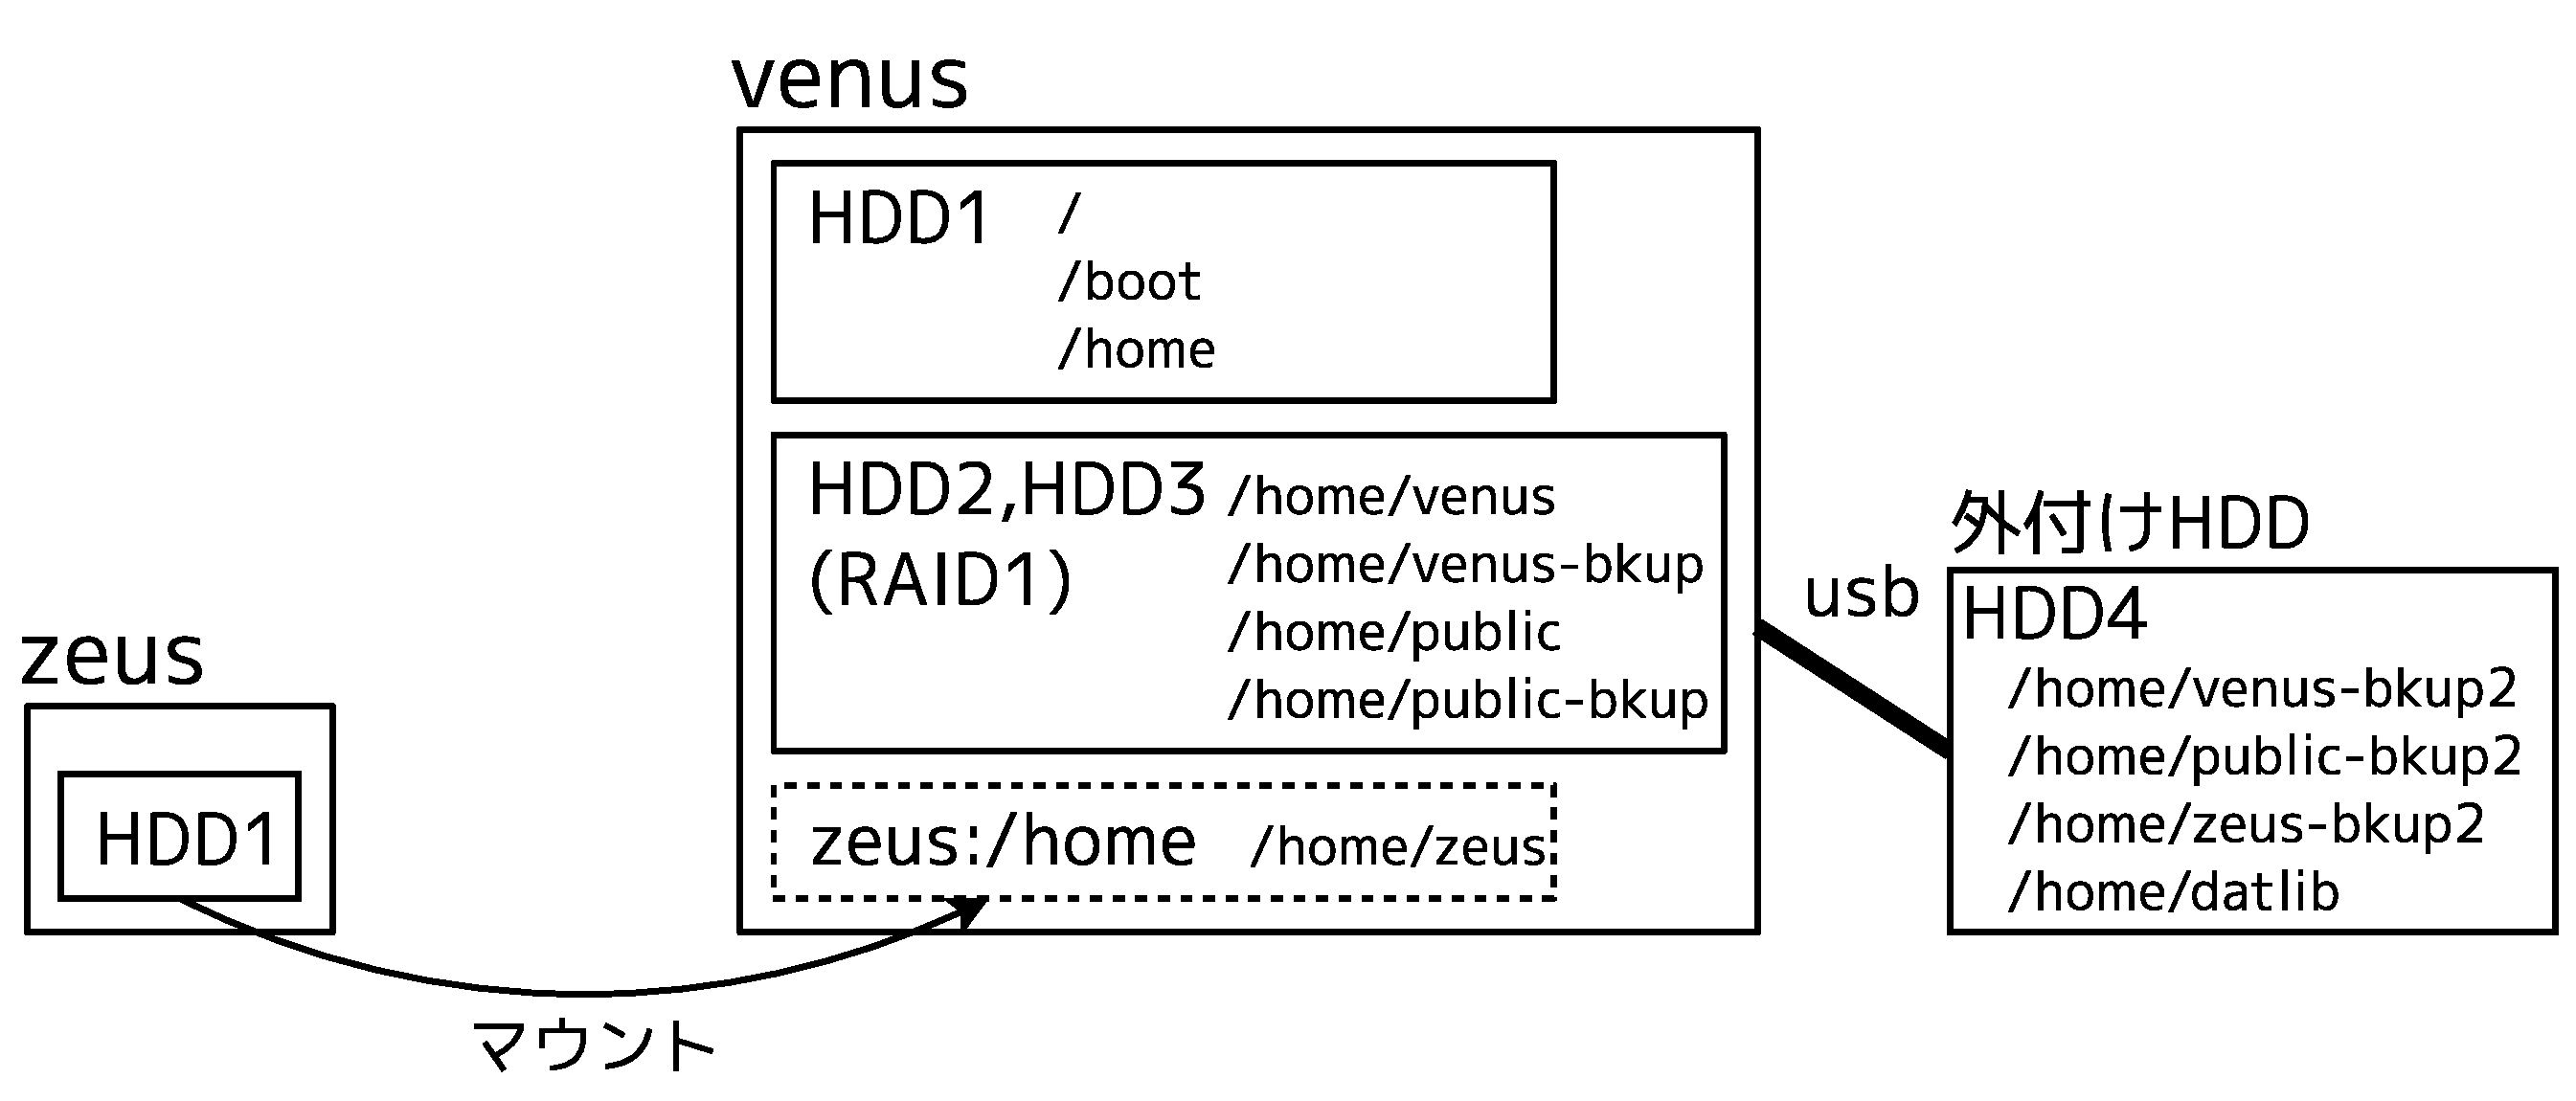
\includegraphics[clip]{bkup-images/venus-hdd.eps}}
%    \vspace*{0.1cm}
    \caption{venusのディスク構成 \label{fig:venus-hdd}}
  \end{center}
\end{figure}



\subsection{zeus編}

zeusのディスク構成は図2のようになっています。


\begin{itemize}
\item HDD1 : zeus内ハードディスク \\
      サーバに必要な機能のほか、/home以下に研究室のHPやみんなに届いたメールなどが入っている
\item HDD2 : 外付けハードディスク \\
      毎日のバックアップ先
\end{itemize}


\begin{figure}[h]
  \begin{center}
    \scalebox{0.38}{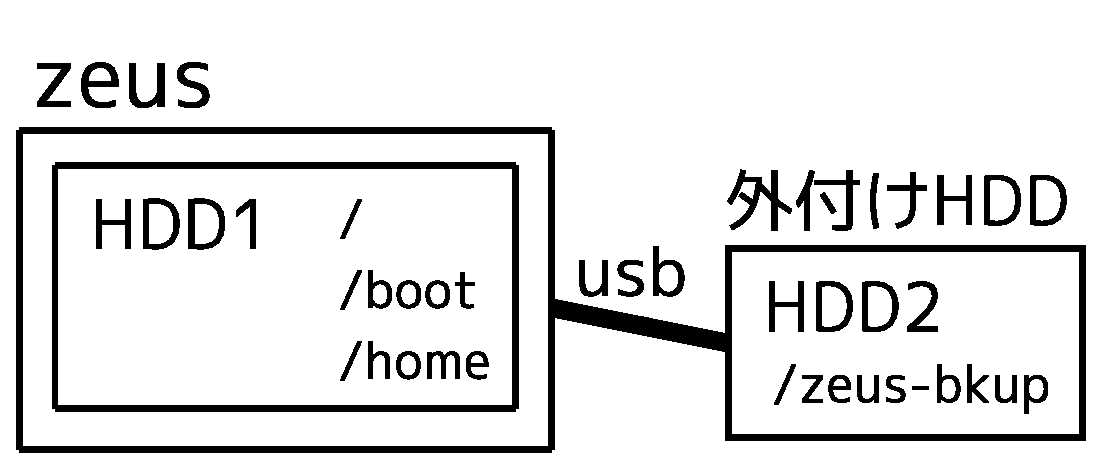
\includegraphics[clip]{bkup-images/zeus-hdd.eps}}
%    \vspace*{0.1cm}
    \caption{zeusのディスク構成 \label{fig:zeus-hdd}}
  \end{center}
\end{figure}



\section{バックアップ情報}

研究室では以下の3つの方法でバックアップを行っています。
\begin{itemize}
\item RAIDによるバックアップ
\item cronによるバックアップ
\item DVDによるバックアップ(手動で実行)
\end{itemize}



\subsection{RAIDによるバックアップ}

RAIDとは複数のハードディスクを一枚のハードディスクのように扱う技術で、
その一種であるRAID1(ミラーリング)では、2枚のハードディスクの内容を全く同じに保つことができます。
それにより、片方のハードディスクが壊れた場合でももう1枚を使ってシステムを復旧することができます。

研究室ではvenus内のハードディスク2枚 (図1:HDD2,3)をRAID1にしています
(OSの機能で実現するソフトウェアRAID)。


\if 0 %コメントアウト
\begin{itemize}
\item venus内ソフトウェアRAID (図1:HDD2,3)
\item 外付けハードウェアRAID (venusにUSB接続) (図1:HDD4,5) %外付けRAIDはなくなりました!(2012年現在)
\end{itemize}
\fi


\subsection{cronによるバックアップ \label{sub:cron}}

cronとは、ある日にちや時間になると登録しておいたプログラム(シェルスクリプト)を自動的に実行するサービスです。
/etc/crontabで指定した時間に、指定したスクリプトが実行されます。

cronで実行しているバックアップ用スクリプトは実行情報をadmin(=機械係)にメールで送るようになっているので、
届いたメールできちんと実行されているかチェックしてください。


\subsubsection{venus編 \label{subsub:cron_venus}}

venusで自動実行されているバックアップシェルのリストです。
矢印で示しているのがデータのコピー元とコピー先で、各シェルの置いてある場所は/home/venus/adm/binです。


\begin{itemize}
\item 毎日
\begin{verbatim}
	・bkup_venus.sh : /home/venus → /home/venus-bkup
	・bkup_public.sh : /home/public → /home/public-bkup
\end{verbatim}
\item 毎週土曜
      \begin{verbatim}
	・bkup_venus2.sh : /home/venus → /home/venus-bkup2
	・bin/bkup_public2.sh : /home/public → /home/public-bkup2
	・bin/bkup_zeus2.sh : /home/zeus → /home/zeus-bkup2
      \end{verbatim}
\item 毎月1日
      \begin{verbatim}
	・bkup_cfg.sh : /etc,/var/yp → /home/venus/adm/cfg_bkup  (設定ファイルのバックアップ)
	・mkiso_venus.sh : /home/venus-bkup → /home2/bkup-iso  (DVDに焼くためのイメージファイルの作成)
      \end{verbatim}
\end{itemize}


\subsubsection{zeus編}

zeusで実行されている自動バックアップのリストです。
各シェルの置いてある場所は/home/adm/binです。
\begin{itemize}
\item 毎日
\begin{verbatim}
	・bkup_zeus.sh : /home/zeus → /zeus-bkup
\end{verbatim}
\item 毎月1日
      \begin{verbatim}
	・bkup_cfg.sh : /etc → /home/adm/cfg_bkup  (設定ファイルのバックアップ)
      \end{verbatim}
\end{itemize}






\subsection{DVDによるバックアップ}

ハードディスクは壊れやすいので、定期的にDVDに焼いてバックアップします。
このときの操作は手動で行います。
\\

※注意. バックアップ元の圧縮ファイルが4GB以上の場合、分割してDVDに保存されます。


\subsubsection{毎月のバックアップ \label{subsub:dvd_month}}

venusでは毎月1日に、みんなのホームディレクトリをDVDに焼くためのイメージファイル(isoファイル)を作るコマンドを自動実行しています(\ref{subsub:cron_venus}参照)。
venusから実行完了のメール(★)が届いたら、次の操作でisoファイルをDVDに焼きます。

\begin{enumerate}
\item DVD-Rを、1枚では足りないので何枚か用意しておく。
\item venus上でrootになって次のコマンドを実行
      \begin{verbatim}
  # /home/venus/adm/bin/burn_dvd.sh
      \end{verbatim}
\item ''空のDVDをセットしてからキーを押してください''などのメッセージが出るので、画面の指示に従ってDVDを入れ換えたりしてデータを書き込んでいく。
\item データがすべて書き込まれたら''isoファイルを削除しますか(y/n)?''というメッセージが出るので、通常はyを選択して削除する。
\item 最後にDVDのラベルに書く内容が表示されるので、それをDVDに書いておく。
\end{enumerate}

できたDVDはファイルに入れて保存します。
このとき(★)のメールを印刷して一緒に入れておきます。




\subsubsection{半年に1回のバックアップ}

publicとzeusは半年に1回DVDに焼いておきます。
このときはisoファイルを作るコマンドも手動で実行します。
\\

以下はpublicを焼くときの操作方法です。
zeusの場合はコマンドのpublicの部分をzeusにして同じ操作をします。(zeusを焼くときもvenusで操作)
\begin{enumerate}
\item /home2/bkup-isoの中に以前のisoファイルが残ってないことを確認する。
\item venus上でrootになって次のコマンドを実行
      \begin{verbatim}
  # /home/venus/adm/bin/mkiso_public.sh
      \end{verbatim}
\item 後は毎月のバックアップと同じで、burn\_dvd.shを実行させDVDに焼く。
\end{enumerate}



\section*{その他}

図1,2はdiaというソフトで描いたので,ディスク構成が変わったときはdiaで描き直してください(cvs/text/bkup-images/(ファイル名).dia)。



\end{document}




%以下コメントアウト---------------------------------------------------------------

\if 0
\subsubsection*{ 参考. DVDの中身を確認する方法}
焼いた後のDVDを上のコマンドでマウントして、/mnt/tmpに移動して中のファイルを確認する。
\begin{verbatim}
    (rootで)
    # mount -r -t iso9660 /dev/dvd /mnt/tmp
\end{verbatim}
DVDを取り出す前にアンマウントするのを忘れない。
\begin{verbatim}
    # umount /mnt/tmp
\end{verbatim}
\fi



